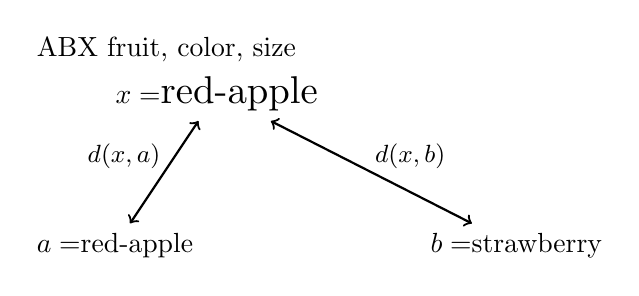
\begin{tikzpicture}[thick]
    \node[anchor=north west] (A) at (0,0) {$a = $\emoji{red-apple}};
    \node[anchor=north west] (X) at (1,2) {$x = $\scalebox{1.4}{\emoji{red-apple}}};
    \node[anchor=north west] (B) at (5,0) {$b = $\emoji{strawberry}};
    \draw[<->] (A) -- node[inner sep=1pt, pos=0.5, above left] {\small $d(x,a)$} (X);
    \draw[<->] (X) -- node[inner sep=1pt, pos=0.5, above right] {\small $d(x,b)$} (B);
    \node[anchor=north west, align=center] at (0, 2.5) {
        ABX \on fruit, \by color, \across size
    };
\end{tikzpicture}